\section{Background}
\begin{figure*}[ht]\centering
	\def\layersep{2cm}
	\def\hiddenlayers{1}
	\def\hiddenneurons{2}
	
	\def\hiddenlayernodes{3}
	
	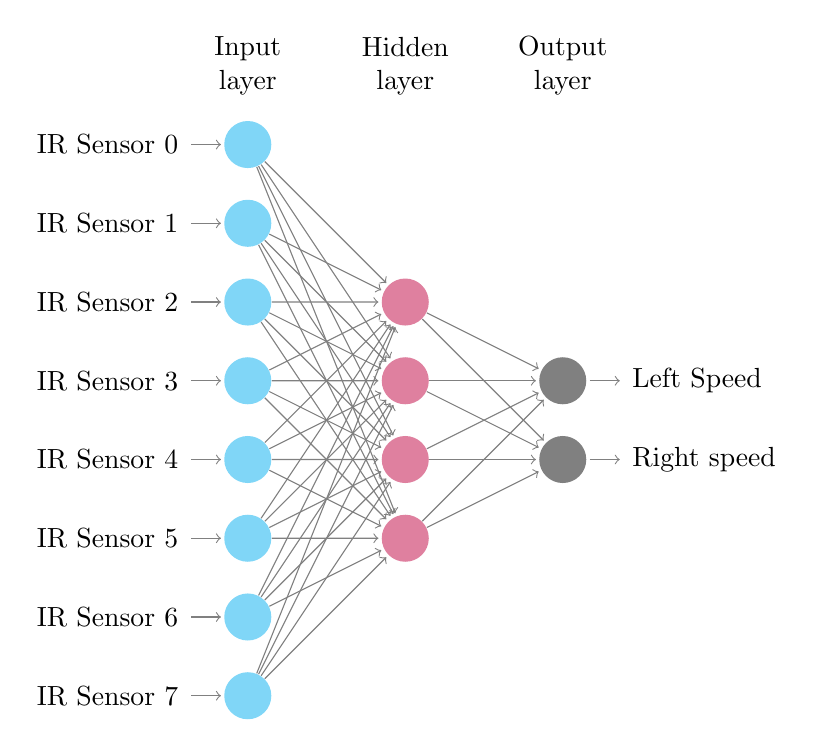
\begin{tikzpicture}[shorten >=1pt,->,draw=black!50, node distance=\layersep]
	\tikzstyle{every pin edge}=[<-,shorten <=1pt]
	\tikzstyle{neuron}=[circle,fill=black!25,minimum size=17pt,inner sep=0pt]
	\tikzstyle{input neuron}=[neuron, fill=cyan!50];
	\tikzstyle{output neuron}=[neuron, fill=black!50];
	\tikzstyle{hidden neuron}=[neuron, fill=purple!50];
	\tikzstyle{annot} = [text width=4em, text centered]
	
	% Draw the input layer nodes
	\foreach \name / \y in {0,...,7}
	% This is the same as writing \foreach \name / \y in {1/1,2/2,3/3,4/4}
	\node[input neuron, pin=left:IR Sensor \y] (I-\name) at (0,-\y) {};
	
	% Draw the hidden layer nodes
	\foreach \name / \y in {0,...,\hiddenlayernodes}
	\path[yshift=-2cm]
	node[hidden neuron] (H-\name) at (\layersep,-\y cm) {};
	
	
	% Draw the output layer node
	\node[yshift=0][output neuron,pin={[pin edge={->}]right:Left Speed}, right of=H-1] (O-1) {};
	\node[yshift=0][output neuron,pin={[pin edge={->}]right:Right speed}, right of=H-2] (O-2) {};
	
	% Connect every node in the input layer with every node in the
	% hidden layer.
	\foreach \source in {0,...,7}
	\foreach \dest in {0,...,\hiddenlayernodes}
	\path (I-\source) edge (H-\dest);
	
	
	% Connect every node in the second hidden layer with the output
	\foreach \source in {0,...,\hiddenlayernodes}
	\foreach \dest in {1,...,2}
	\path (H-\source) edge (O-\dest);
	
	% Annotate the layers
	\node[xshift=0cm][annot,above of=I-1] (first) {Input layer};
	\node[xshift=1cm][annot,right of=first, node distance=1cm] (hl) {Hidden layer};
	\node[xshift=1cm][annot,right of=hl, node distance=1cm] (ll) {Output layer};
	\end{tikzpicture}
	\caption{Neural network}
	\label{fig:NN}
\end{figure*}
%------------------------------------------------

\begin{figure*}[ht]\centering % Using \begin{figure*} makes the figure take up the entire width of the page
\includegraphics[width=\linewidth]{view}
\caption{Wide Picture}
\label{fig:view}
\end{figure*}

%\begin{enumerate}[noitemsep] % [noitemsep] removes whitespace between the items for a compact look
%\item First item in a list
%\item Second item in a list
%\item Third item in a list
%\end{enumerate}

\subsection{Elevated Plus Maze}

\subsubsection*{History} 
Initially conceived in 1955 by K. C. Montgomery as a way to study the simultaneous feelings of curiosity and fear that rats experience when exposed to a new environment.
\paragraph{Paragraph} test % Dummy text

\subsection{Genetic Algorithm}

test % Dummy text

\subsection{Neural Network}

Reference to Figure \ref{fig:NN}.

%------------------------------------------------

